\section{The ZFOURGE Survey} \label{Sec: The ZFOURGE Survey}
\subsection{Overview}
This study utilises the 2017 release\footnote{Available for download at \href{https://zfourge.tamu.edu/}{zfourge.tamu.edu.}} of the ZFOURGE survey \citep{straatman_fourstar_2016}, which offers a unique combination of depth and wavelength coverage essential for probing high-redshift galaxies and constructing accurate LFs. ZFOURGE consists of approximately 70,000 galaxies at redshifts greater than 0.1 covering three major 11$\times$11 arcminute fields: the Chandra Deep Field South (CDFS) \citep{giacconi_chandra_2002}, the field observed by the Cosmic Evolution Survey (COSMOS) \citep{scoville_cosmic_2007}, and the CANDELS Ultra Deep Survey (UDS) \citep{lawrence_ukirt_2007}. These galaxies were observed using the near-infrared FourStar imager \citep{persson_fourstar_2013} mounted on the 6.5-m Magellan Baade Telescope at the Las Campanas Observatory in Chile. 

ZFOURGE employs deep near-infrared imaging with multiple medium-band filters (\textit{J}$_{1}$, \textit{J}$_2$, \textit{J}$_{3}$, \textit{H}$_{l}$, \textit{H}$_{s}$) and a broad-band \textit{K}$_{s}$ filter. The imaging spans 1.0 to 1.8 $\mu$m and achieves 5$\sigma$ point-source limiting depths of 26 AB mag in the \textit{J} medium-bands and 25 AB mag in the \textit{H} and \textit{K}$_{s}$ bands \citep{spitler_first_2012}. These filters yield well-constrained photometric redshifts, particularly effective for sources within the redshift range of 1 to 4 \citep{spitler_first_2012}. ZFOURGE data is supplemented by public data from HST/WFC3 F160W and F125W imaging from the CANDELS survey, Spitzer/Infrared Array Camera (IRAC), and Herschel/Photodetector Array Camera and Spectrometer (PACS). For a detailed description of the data and methodology, refer to \cite{straatman_fourstar_2016}.

\subsection{Sample Selection} \label{Sec: Sample Selection}
To ensure the selection of high-quality galaxies and minimise errors in our analysis, we adopt the ZFOURGE quality flag \texttt{Use=1}, as defined by \cite{straatman_fourstar_2016}. This flag selects galaxies with reliable photometry and redshift measurements, resulting in a starting sample of 37,647 galaxies. We refine the sample by removing sources with unphysical bolometric luminosities ($L_{bol} < 0$), which reduces the sample to 22,967 galaxies.

\subsubsection{ZFOURGE total \& Decomposed SF Sample} \label{Sec: Galaxy LF Selection}
Next, we use the ZFOURGE AGN catalogues \citep{cowley_zfourge_2016} to identify and exclude 552 AGN-dominated sources to prevent AGN contamination of the luminosity functions. After excluding these AGN sources, we apply a redshift cut, restricting the sample to $0 \leq z \leq 6$ since only 28 galaxies exist at $z > 6$. This redshift range enables us to observe the evolution of galaxies during some of the most critical cosmic periods, specifically around $1 < z < 3$ \citep{gruppioni_modelling_2011, wylezalek_galaxy_2014} where galaxy luminosity density peaks \citep{assef_mid-ir-_2011}. This sample includes 22,444 galaxies, which we use to construct the ZFOURGE total and CIGALE SF LFs.

To ensure robustness, we calculate the bolometric flux from the bolometric luminosity of each sample and apply an 80\% completeness cut. This reduces the impact of noise and observational limits while preserving a large enough sample for LF construction. We also apply a completeness cut that requires the maximum observable volume of each galaxy to extend to the end of the redshift bin. These completeness cuts reduce the final LF sample to 16,154 galaxies.

\subsubsection{Decomposed AGN Sample} \label{Sec: Decomposed AGN Selection}
Although AGN-dominated sources are removed from the ZFOURGE galaxy and CIGALE SF sample, they are retained for separate analysis to construct decomposed AGN LFs through SED decomposition. For a comprehensive explanation of the SED decomposition process, please refer to Section \ref{Sec: CIGALE}. For this AGN-specific analysis, we include all sources with a significant AGN fraction ($\mathcal{F}_{AGN}>0.1\ L_{AGN}/L_{bol}$); 12,390 sources. Applying the same luminosity completeness cut and 80\% completeness cut to the bolometric flux, the AGN sample is reduced to a final set of 8,800 galaxies spanning $0 \leq z \leq 6$. Figure \ref{Fig: ZF Lum vs z} shows the reduced luminosity-redshift distribution of ZFOURGE (top), CIGALE AGN (middle), and CIGALE SF (bottom).

\begin{figure}
    \centering
    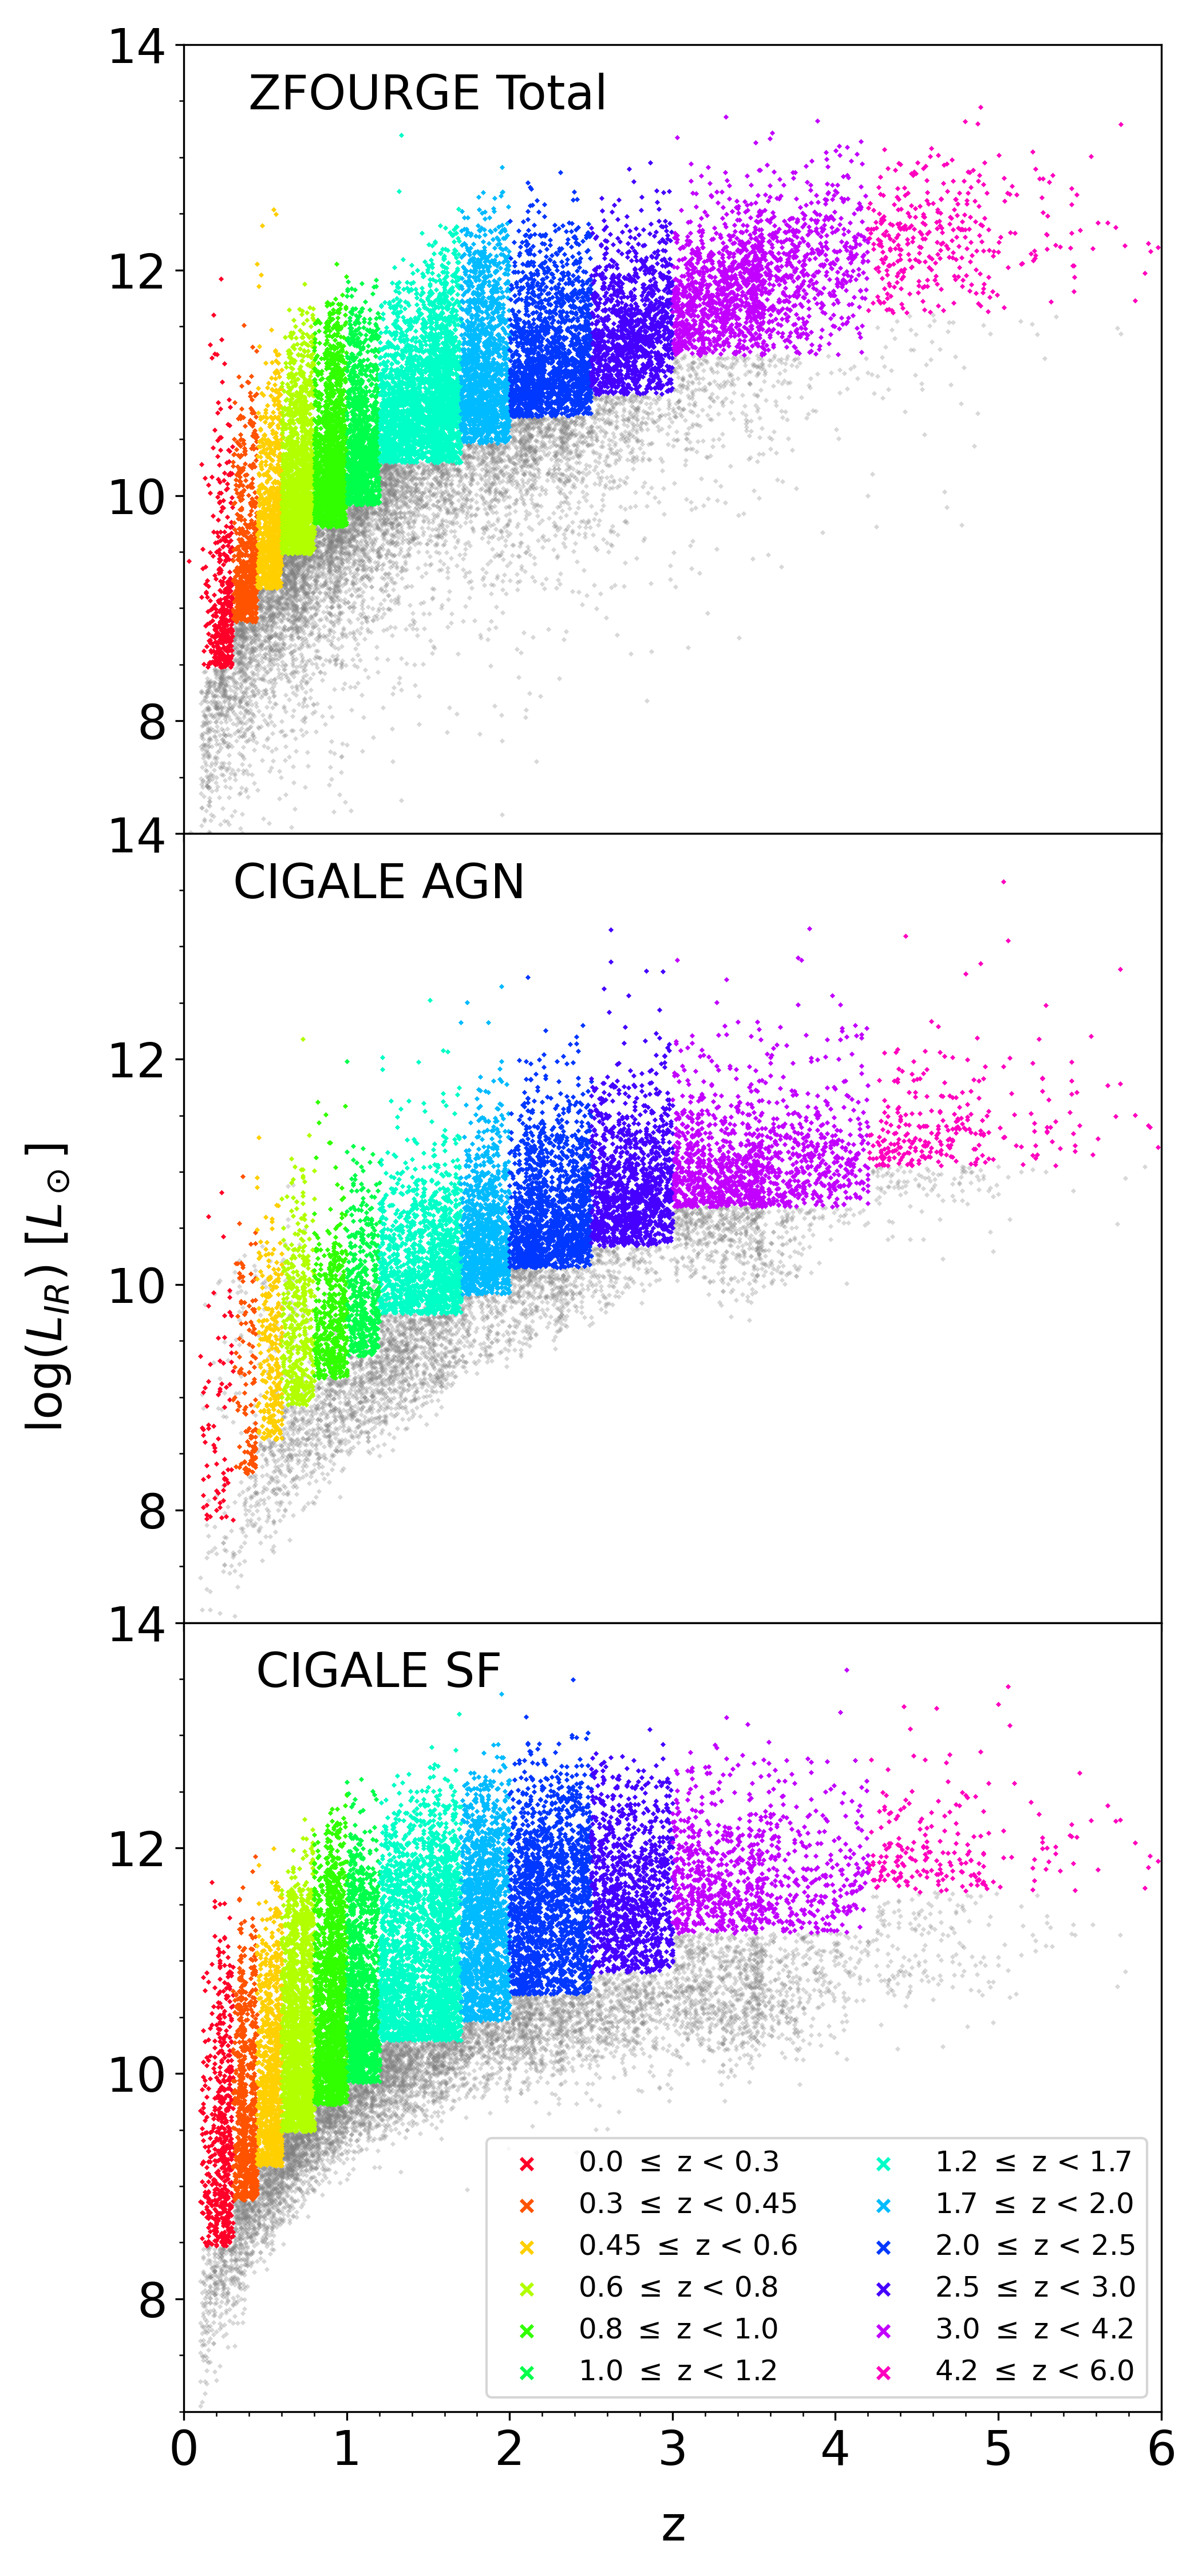
\includegraphics[width=0.7\textwidth]{Figures/LIR_vs_Z.png}
    \caption{Luminosity-redshift distributions of (top) the ZFOURGE bolometric $8-1000\mu m$ luminosity, (middle) the CIGALE AGN luminosity, and (bottom) the CIGALE SF luminosity. Sources are coloured by redshift bin or coloured grey if removed as described in section \ref{Sec: Sample Selection}}
    \label{Fig: ZF Lum vs z}
\end{figure}

\section{Decomposing Galaxy SEDs} \label{Sec: CIGALE}
The public version of the ZFOURGE catalogues has utilised \texttt{EAZY} \citep{brammer_eazy_2008} and \texttt{FAST} \citep{kriek_ultra-deep_2009} for parameterising galaxy properties, primarily focusing on photometric redshifts, stellar masses, and SFRs. However, while effective, these methods provide a more generalised view of galaxy properties without entirely disentangling the contributions from different physical components within each galaxy, such as SF regions and AGN. To address this limitation, we employ the SED fitting software CIGALE \citep{boquien_cigale_2019}, which enables the decomposition of observed light from galaxies into distinct components, including SF and AGN activity. This method builds on the work by \cite{cowley_decoupled_2018}, incorporating additional photometric coverage and an updated parameter space to better quantify AGN contributions.

\subsection{CIGALE Methodology and Parameter Space} \label{Sec: CIGALE_Parameters}
CIGALE performs multi-component SED fitting to derive galaxy properties by integrating our photometry from 0.2 $\mu$m to 160 $\mu$m across the CDFS field and up to 24 $\mu$m for COSMOS and UDS. This broader wavelength coverage allows for a more complete and precise decomposition of galaxy light into SF and AGN components. The decomposition uses a range of parameter values (see Table \ref{tab:parameter_space}), allowing for flexible modelling of star formation histories (SFH), dust attenuation, AGN torus contributions, and other factors. We also incorporate the SKIRTOR AGN torus model \citep{stalevski_dust_2016}, which better handles clumpy dust distributions and polar dust extinction, providing an accurate characterisation of AGN emission.

\subsection{Bolometric IR Luminosity Derivation} \label{Sec: IR_Luminosity}
Understanding the total IR energy output of galaxies is essential for tracing both SF and AGN activity, particularly in dusty environments where much of the energy is re-emitted in the IR \citep{fu_decomposing_2010}. By estimating the bolometric IR luminosity, we can gain insights into the contribution of these processes across cosmic time. 

For the ZFOURGE total LF sample, we adopted the approach in \cite{straatman_fourstar_2016} where the averaged \cite{wuyts_fireworks_2008} template was fit to the 24-160 $\mu$m photometry to estimate the total bolometric IR luminosity. This method provides a robust measure of the IR emission for purely star-forming galaxies without AGN contamination.

For the Decomposed SF and AGN LF samples, we derive luminosities through a different approach. CIGALE performs SED decomposition on the entire galaxy emission, using its integrated models to separate the total luminosity into distinct stellar, dust, and AGN components. The stellar and dust luminosities are combined to form the SF component, while the AGN component is derived directly from CIGALE's emission modelling. These distinct approaches are subsequently used to construct the IR luminosity functions of the two samples. 

Figure \ref{Fig: LIR vs LIR} compares the CIGALE total luminosity to the ZFOURGE total bolometric luminosity ($L_{bol}$). In the top panel, galaxies are coloured based on their redshift bin. It can be seen that the brightest galaxies are more likely to exist at higher redshifts. In the bottom panel, galaxies are coloured based on the AGN fraction ($\mathrm{F}_{AGN}$) to the total luminosity derived by CIGALE. Galaxies at higher redshift are brighter and more likely to host a powerful AGN.

\begin{table}[htbp]
    \caption{Parameter space used for SED fitting with CIGALE}
    \label{tab:parameter_space}
    \begin{center}
    \begin{tabular}{ll}
        \toprule
        \textbf{Parameter} & \textbf{Model/Values} \\ 
        \hline
        SFH                 & Delayed SFH $\tau = 1,3,5,7,9,11$ Gyr \\
        Age                 & $0.5, 1, 3, 5, 7, 9, 11$ Gyr \\
        Burst Fraction      & $0.0, 0.01, 0.05, 0.1, 0.15, 0.2, 0.3$ \\
        SSP                 & \cite{bruzual_stellar_2003} \\
        IMF                 & \cite{chabrier_galactic_2003} \\
        Metallicity         & Fixed at 0.02 \\
        Nebular             & \cite{inoue_rest-frame_2011} \\
        Dust Atten.         & \cite{calzetti_dust_2000} $E_{(B-V)} = 0.01, 0.05, 0.1, 0.5$, \\
                            & $1.0, 1.5$ \\
        Dust Emission       & \cite{dale_two-parameter_2014} $\alpha = 1.0, 1.5, 2.0, 2.5, 3.0$ \\
        AGN Model           & SKIRTOR \citep{stalevski_3d_2012, stalevski_dust_2016} \\
        Torus Inclination   & $30^\circ, 70^\circ$ \\
        AGN Fraction        & $0.0, 0.01, 0.1 - 0.9$ (steps of 0.1), 0.99 \\
        Polar Extinction    & SMC $E(B-V) = 0.0, 0.03, 0.1, 0.2, 0.4, 0.6, 1.0, 1.8$ \\
        \bottomrule
    \end{tabular}
    \end{center}
\end{table}

\begin{figure}
    \centering
    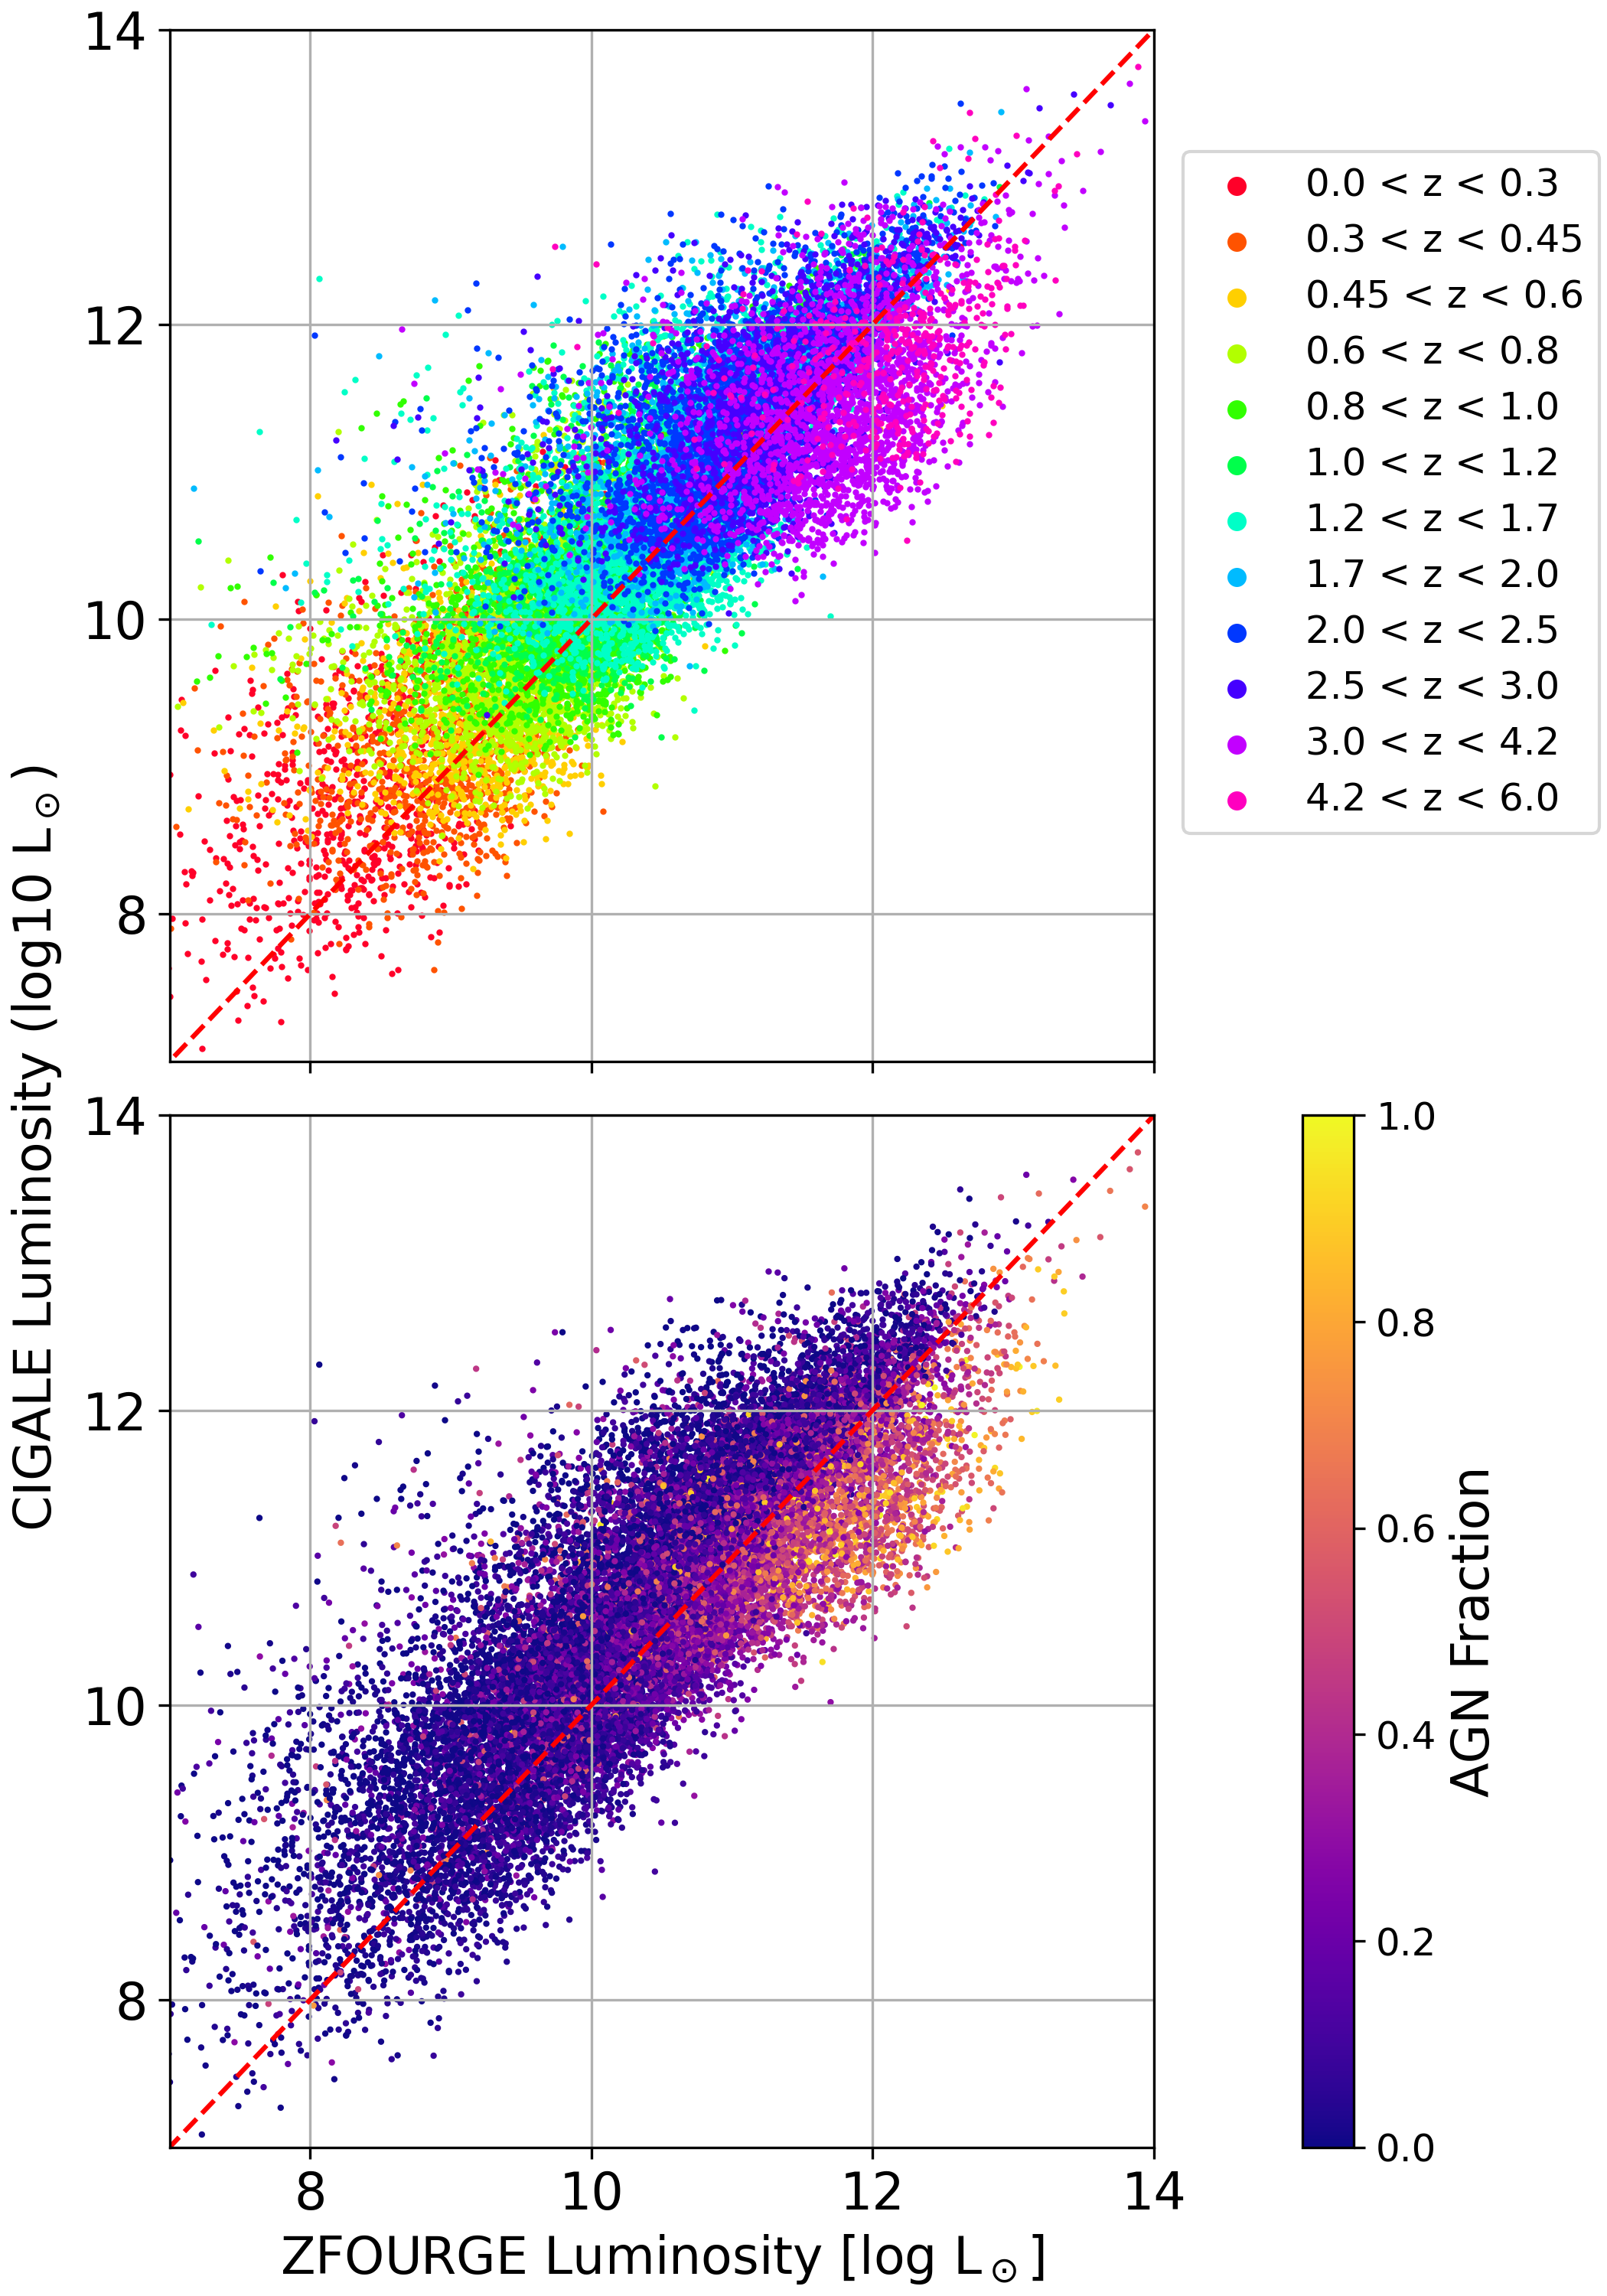
\includegraphics[width=0.9\textwidth]{Figures/LIR_vs_LIR.png}
    \caption{ZFOURGE bolometric 8-1000$\mu$m IR luminosity compared to CIGALE total luminosity. Top: Sources coloured by redshift bin. Bottom: sources coloured by AGN fraction ($\mathcal{F}_{AGN}$). AGN fraction increases with redshift. At $z \geq 3$, the average AGN fraction is greater than 30\%.}
    \label{Fig: LIR vs LIR}
\end{figure}

\subsection{Robustness Tests with Mock Analysis} \label{Sec: Mock_Analysis}
To ensure the reliability of the decomposition process, particularly for faint AGN, we performed a series of robustness tests using CIGALE's built-in mock analysis. These tests evaluate the software's ability to accurately decompose AGN and SF contributions across various redshifts and luminosities, specifically focusing on galaxies with low bolometric luminosities. By comparing the input and recovered AGN luminosities from the analysis, we confirmed that our parameter space and methodology are robust, particularly in detecting faint AGN. The mock analysis demonstrated that AGN luminosity was reliably constrained, with Pearson correlation coefficients (PCCs) ranging from 0.969 to 0.973 across all fields. Most sources lay within 0.5 dex of the 1-to-1 line, with mean residuals between $-0.02$ and $0.04$ dex, confirming the robustness of AGN luminosity recovery. These results indicate that our method effectively minimises bias against faint AGN, which are often difficult to detect in traditional analyses.

For a more comprehensive description of the SED decomposition methodology, see \cite{cowley_decoupled_2018}. Additionally, refer to the CIGALE software paper \citep{boquien_cigale_2019} for detailed information on its decomposition process and parameter optimisation techniques.

